\documentclass{article}

% Packages for formatting
\usepackage{tcolorbox}
\usepackage{xcolor}
\usepackage{hyperref}
\usepackage{amsmath}
\usepackage{geometry}
\usepackage{tocloft}
\usepackage{colortbl}
\usepackage{graphicx}
\usepackage{lipsum} % For dummy text

% Change hyperref settings to remove boxes
\hypersetup{
    colorlinks=true,
    linkcolor=black,
    filecolor=black,
    urlcolor=black,
    citecolor=black,
}

% Page layout
\geometry{a4paper, margin=1in}

% Colors
\definecolor{codehighlight}{rgb}{0.36, 0.54, 0.66}
\definecolor{coderule}{rgb}{0.7, 0.7, 0.7}           % Grey frame codebox
\definecolor{codebg}{rgb}{1.0, 1.0, 1.0}             % Background codebox
\definecolor{tableheader}{RGB}{128, 128, 128}        % Grey table header
\definecolor{tablecell}{RGB}{250, 250, 250}          % Table cell
\definecolor{title}{rgb}{0.36, 0.54, 0.66}           % Custom title color


% Code box style
\tcbset{
    colframe=tableheader, % Frame color
    colback=tablecell,    % Background color
    arc=0pt,           % Corner radius
    boxrule=1pt        % Frame thickness
}

% Table of contents
% \renewcommand{\cftbot}{}

% Main document
\begin{document}

% Cover pages
% Cover page
\begin{titlepage}
    \centering
    \vspace{\fill}  % push everything to top

    \thispagestyle{empty} % Remove page numbering

    % Background image
    \newgeometry{left=0cm, right=0cm, top=0cm, bottom=0cm} % Temporarily set margins to 0
    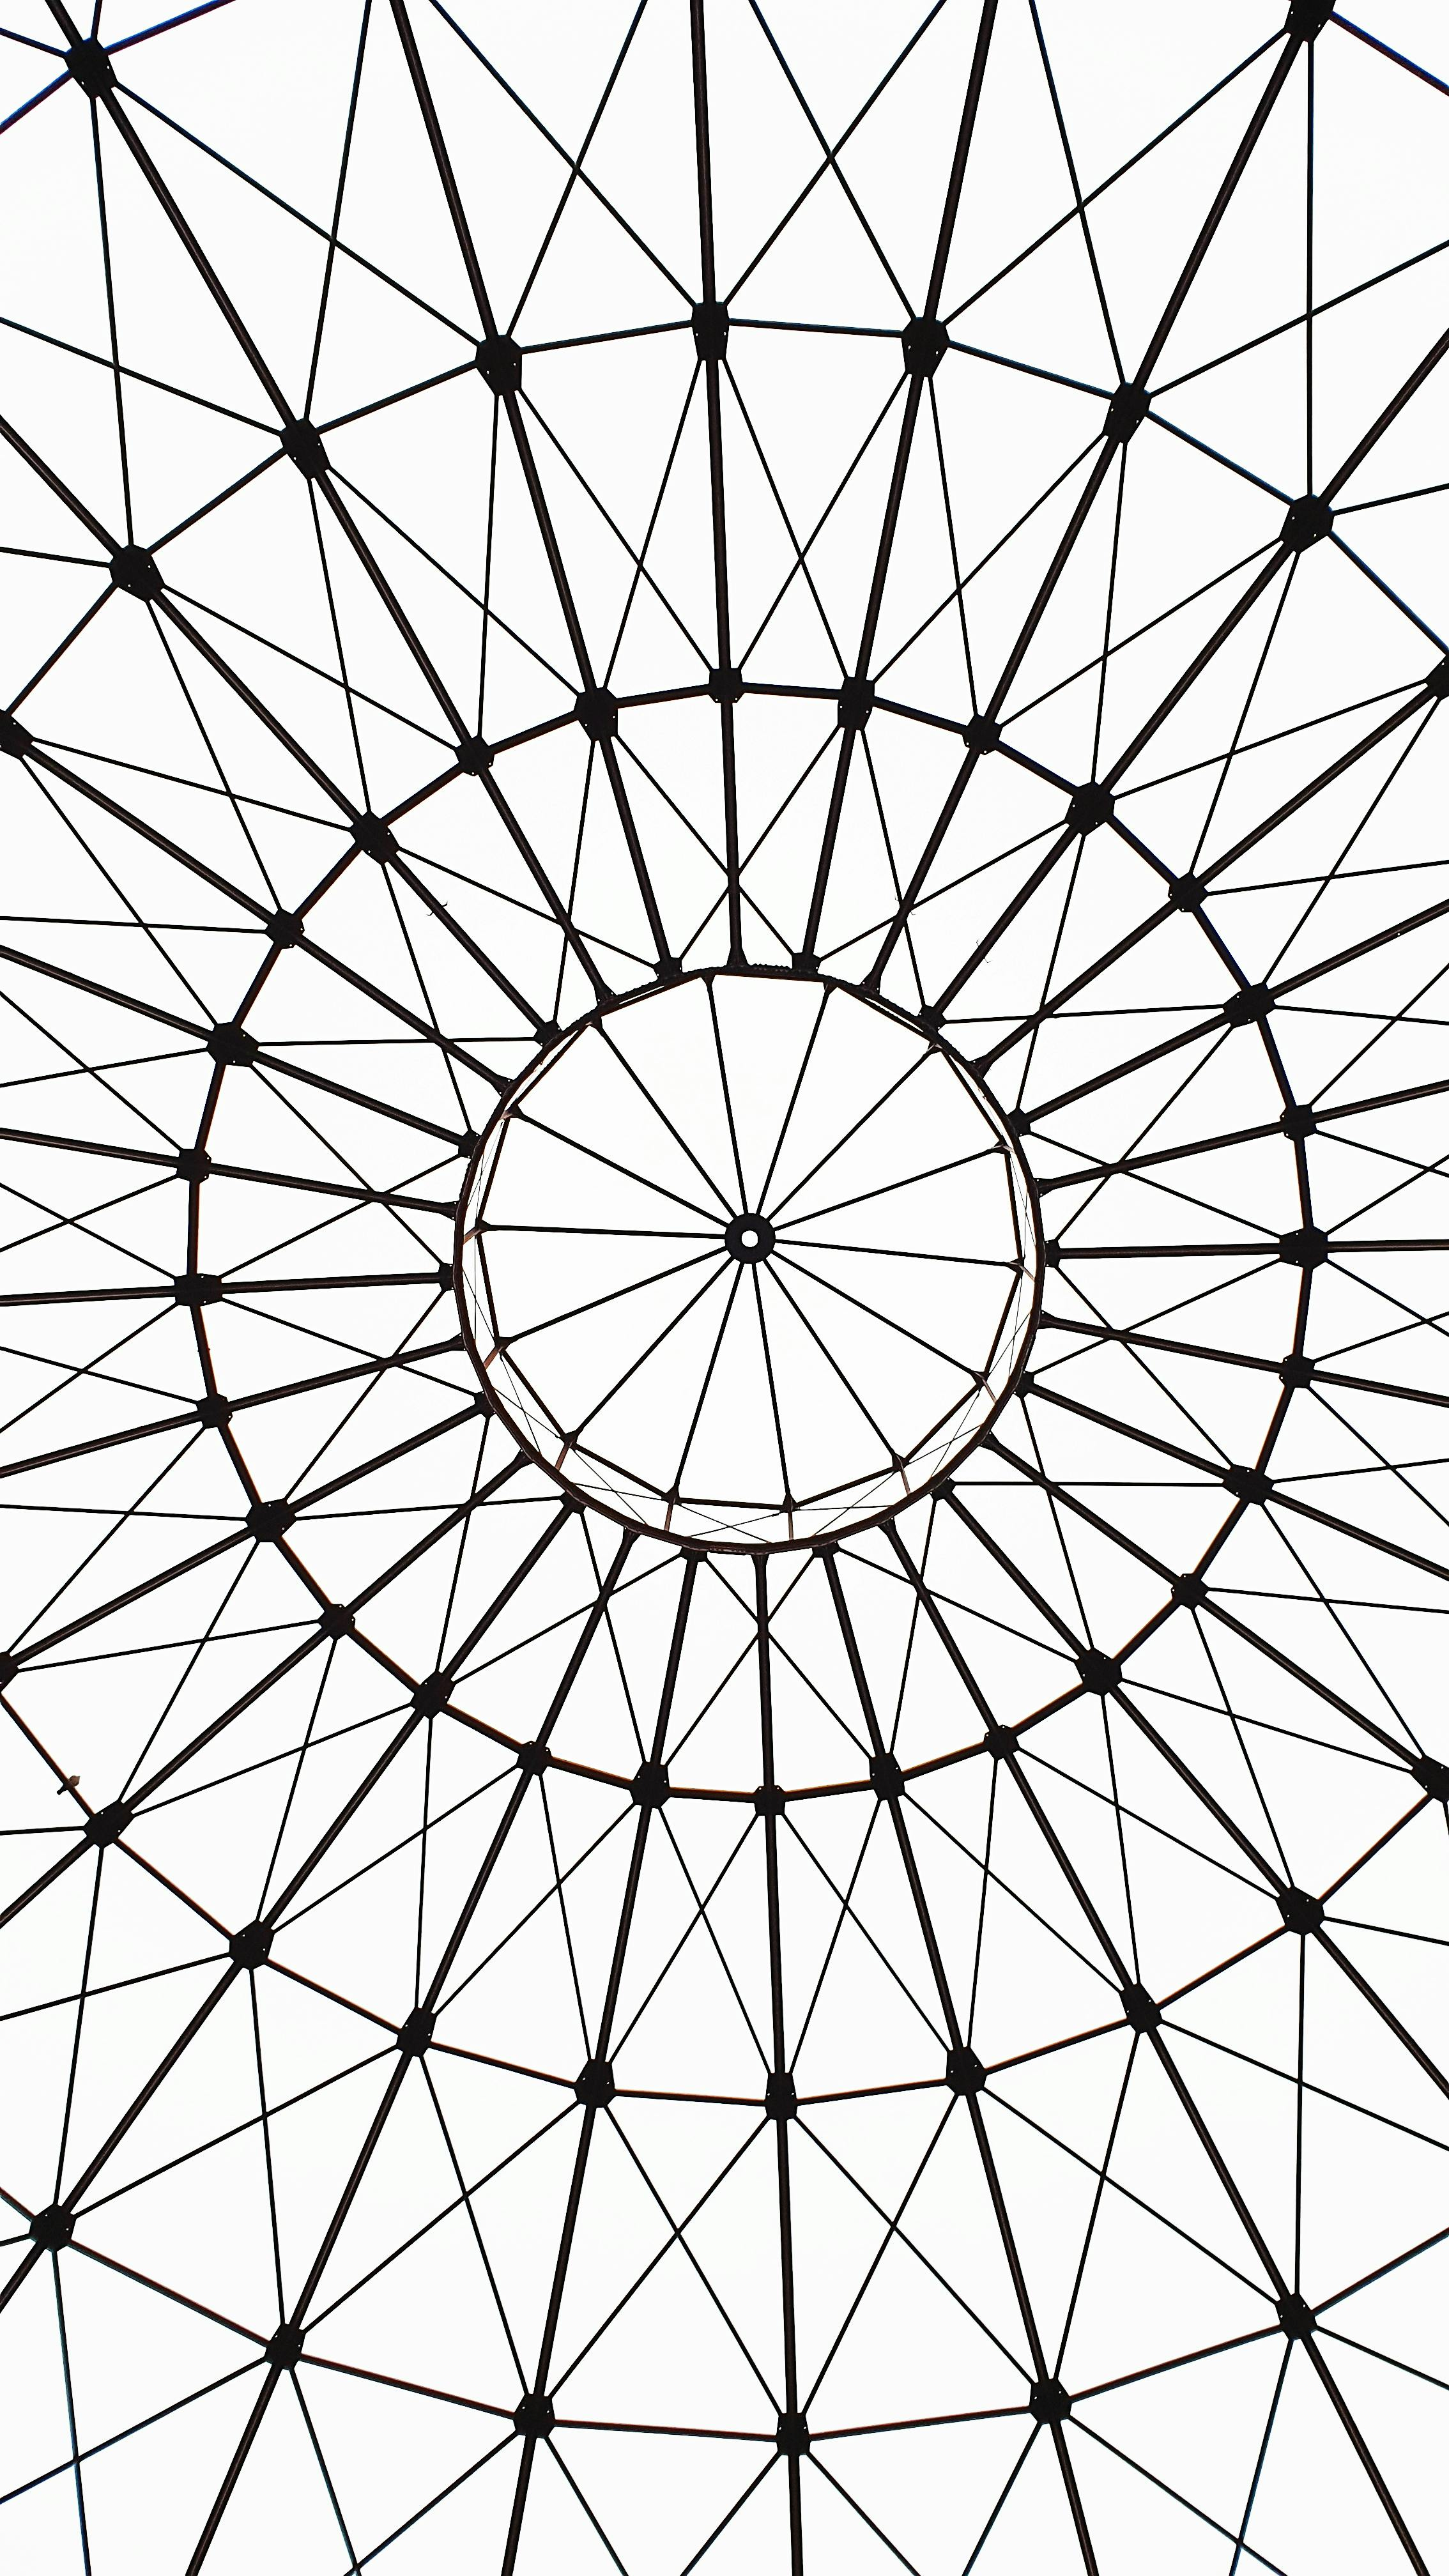
\includegraphics[width=\paperwidth,height=\paperheight]{images/cover.jpg}
    \restoregeometry % Restore the margins

    \vspace{\fill}   % push everything to bottom
\end{titlepage}
\newpage
\ % The empty page
\thispagestyle{empty} % Remove page numbering
\newpage
% Title page
\begin{titlepage}
    \thispagestyle{empty} % Remove page numbering
    \centering
    \vfill                % push everything to top
    \begin{center}
        {\Huge \textbf{My QuestionBook Template}}\\
        \vspace{1cm}
        {\Large Anchit Mulye}\\
        \vspace{0.5cm}
        {\Large \today}
    \end{center}
    \vfill                % push everything to bottom
\end{titlepage}
\newpage
\ % The empty page
\thispagestyle{empty} % Remove page numbering
\newpage
\pagenumbering{roman}
% Table of contents
\newpage
\thispagestyle{empty} % Remove page numbering
\title{My Notebook Template}
\author{Anchit Mulye}
\date{\today}
\maketitle

\tableofcontents
\newpage

% Chapters
\pagenumbering{arabic}
\section{Introduction}

% Lorem Ipsum is simply dummy text of the printing and typesetting industry. Lorem Ipsum has been the industry's standard dummy text ever since the 1500s, when an unknown printer took a galley of type and scrambled it to make a type specimen book. It has survived not only five centuries, but also the leap into electronic typesetting, remaining essentially unchanged. It was popularised in the 1960s with the release of Letraset sheets containing Lorem Ipsum passages, and more recently with desktop publishing software like Aldus PageMaker including versions of Lorem Ipsum.

\lipsum[1] % Dummy text for illustration

\subsection{Main Section}
\lipsum[2] % Dummy text for illustration

\subsubsection{Subsection}
\lipsum[3] % Dummy text for illustration

\paragraph{Paragraph Heading}
This is a paragraph with a heading. It provides a way to further organize content within a subsection or subsubsection.

\lipsum[4] % Dummy text for illustration

\subsection{Another Main Section}
\lipsum[5] % Dummy text for illustration

\paragraph{Another Paragraph Heading}
This is another paragraph with a heading. You can use multiple paragraph headings within a subsection or subsubsection to structure your content.

\lipsum[6] % Dummy text for illustration

\lipsum[7] % Dummy text for illustration

\lipsum[8] % Dummy text for illustration

\lipsum[9] % Dummy text for illustration
\section{Mathematical Equations}

Some mathematical equations:

\begin{equation}
    E = mc^2
\end{equation}

\begin{equation}
    \frac{d}{dx} \left( e^{x} \right) = e^{x}
\end{equation}

\begin{equation}
    \int_{a}^{b} x^2 \, dx = \left[ \frac{x^3}{3} \right]_{a}^{b}
\end{equation}

\begin{equation}
    \vec{F} = m \vec{a}
\end{equation}

\begin{equation}
    \sigma = \frac{F}{A}
\end{equation}

\begin{equation}
    \sum_{n=1}^{N} n = \frac{N(N+1)}{2}
\end{equation}
\section{Programming}

This is a coding section using tcolorbox for code examples.

\subsection{Python Code}
\begin{tcolorbox}[title=Python Code Example]
\begin{verbatim}
def hello_world():
    print("Hello, World!")
\end{verbatim}
\end{tcolorbox}

\subsection{C++ Code}
\begin{tcolorbox}[title=C++ Code Example]
\begin{verbatim}
#include <iostream>

int main()
{
    std::cout << "Hello, World!" << std::endl;
}
\end{verbatim}
\end{tcolorbox}

\subsection{JavaScript Code}
\begin{tcolorbox}[title=JavaScript Code Example]
\begin{verbatim}
function helloWorld() {
    console.log("Hello, World!");
}
\end{verbatim}
\end{tcolorbox}
\section{Text Formatting}

This section contains various text formatting settings in Latex.

\subsection{Font Styles}

\textbf{This is bold text.}\\
\textit{This is italic text.}\\
\underline{This is underlined text.}\\
\texttt{This is typewriter (monospaced) text.}\\
\textsc{This is small caps text.}\\
\emph{This is emphasized text.}

\subsection{Font Sizes}

\tiny{This is tiny text.}\\
\scriptsize{This is scriptsize text.}\\
\footnotesize{This is footnotesize text.}\\
\small{This is small text.}\\
\normalsize{This is normal size text.}\\
\large{This is large text.}\\
\Large{This is larger text.}\\
\LARGE{This is even larger text.}\\
\huge{This is huge text.}\\
\Huge{This is hugest text.}

\subsection{Text Colors}

\textcolor{red}{This is red text.}\\
\textcolor{blue}{This is blue text.}\\
\textcolor{green}{This is green text.}\\
\textcolor{codehighlight}{This is custom color text.}

\subsection{Combined Formatting}

\textbf{\textit{This is bold and italic text.}}\\
\underline{\textbf{\textit{This is bold, italic, and underlined text.}}}\\
\textcolor{blue}{\textbf{This is bold blue text.}}
\section{Tables}

% Normal Table
\subsection{Simple Table}
\begin{table}[h]
\centering
\begin{tabular}{|>{}c|c|c|}
\hline
\rowcolor{tableheader}
\textbf{Column 1} & \textbf{Column 2} & \textbf{Column 3} \\
\hline Item 1 & Item 2 & Item 3 \\
\hline Item 4 & Item 5 & Item 6 \\
\hline
\end{tabular}
\caption{A simple table}
\end{table}

\subsection{Colored Table}
\begin{table}[h]
\centering
\begin{tabular}{|>{\columncolor{tableheader}}c|c|c|}
\hline
\rowcolor{tableheader}
\textbf{Column 1} & \textbf{Column 2} & \textbf{Column 3} \\
\hline Item 1 & Item 2 & \cellcolor{codehighlight} Item 3 \\
\hline Item 4 & \cellcolor{codehighlight} Item 5 & Item 6 \\
\hline
\end{tabular}
\caption{A colored table}
\end{table}

% Headerless table
\subsection{Headless Table}
\begin{center} % This is same as /centering
\normalsize % or \footnotesize, \scriptsize, \tiny
\begin{tabular}{|c|c|c|}
\hline Item 1 & Item 2 & Item 3 \\
\hline Item 4 & Item 5 & Item 6 \\
\hline Item 7 & Item 8 & Item 9 \\
\hline
\end{tabular}
\end{center}

% Borderless table
\subsection{Borderless Table}
\begin{center} % This is same as /centering
\normalsize % or \footnotesize, \scriptsize, \tiny
\begin{tabular}{ccc}
\hline Item 1 & Item 2 & Item 3 \\
\hline Item 4 & Item 5 & Item 6 \\
\hline Item 7 & Item 8 & Item 9 \\
\hline
\end{tabular}
\end{center}

% Complete Borderless table
\subsection{Complete Borderless Table}
\begin{center} % This is same as /centering
\normalsize % or \footnotesize, \scriptsize, \tiny
\begin{tabular}{ccc}
Item 1 & Item 2 & Item 3 \\
Item 4 & Item 5 & Item 6 \\
Item 7 & Item 8 & Item 9 \\
\end{tabular}
\end{center}

% Normal Table color
\subsection{Headless Table with Alternating Row Colors}
\raggedright
\large
\begin{tabular}{|c|c|c|}
\hline
\rowcolor{codehighlight} Item 1 & Item 2 & Item 3 \\
\hline Item 4 & Item 5 & Item 6 \\
\hline
\rowcolor{codehighlight} Item 7 & Item 8 & Item 9 \\
\hline
\end{tabular}

% References Section
\section{References}

\begin{enumerate}

% Book example
\item Smith, J. D. (2009). \textit{The Art of Writing}. Random House.
% Edited book example
\item Smith, A. B. (Ed.). (2010). \textit{Advances in Linguistics}. Cambridge University Press.
% Journal article example (print)
\item Jones, S. C., \& Davis, R. J. (2017). Understanding cultural intelligence. \textit{Journal of Cross-Cultural Psychology, 48}(4), 493-514. \url{https://doi.org/10.1177/0022022117704302}
% Journal article example (online)
\item Roberts, T. F., \& Hidajat, M. (2020). Exploring the impact of social media on adolescent development. \textit{Journal of Adolescent Research, 35}(2), 187-210. \url{https://doi.org/10.1177/0743558420913356}
% Website example with author
\item Davis, M. (2018). Understanding climate change. Retrieved from \url{https://www.example.com/climate-change}
% Website example without author
\item National Institute of Mental Health. (2021). Depression in children and teens. Retrieved from \url{https://www.nimh.nih.gov/health/topics/depression}
% Chapter in edited book example
\item Green, R. T. (2012). Language development in early childhood. In P. H. Smith (Ed.), \textit{Language Acquisition: Theoretical Approaches} (pp. 45-68). Oxford University Press.
% Newspaper article example
\item Smith, J. (2022, June 15). New trends in technology. \textit{The New York Times}, pp. A1, A10.
% Report or government document example
\item United Nations. (2015). \textit{Sustainable Development Goals: 17 Goals to Transform Our World}. Author.
% Conference paper example
\item Brown, L. M. (2019). Education reform in the digital age. Paper presented at the Annual Conference of the American Educational Research Association, Toronto, Canada.
% Thesis or dissertation example
\item Johnson, S. L. (2018). \textit{Understanding leadership in nonprofit organizations} (Doctoral dissertation). Harvard University.

\end{enumerate}



\end{document}